% TraceAssist pipeline, from question to answer. Standalone; build with
%   pdflatex traceassist_pipeline.tex
% and include the PDF with 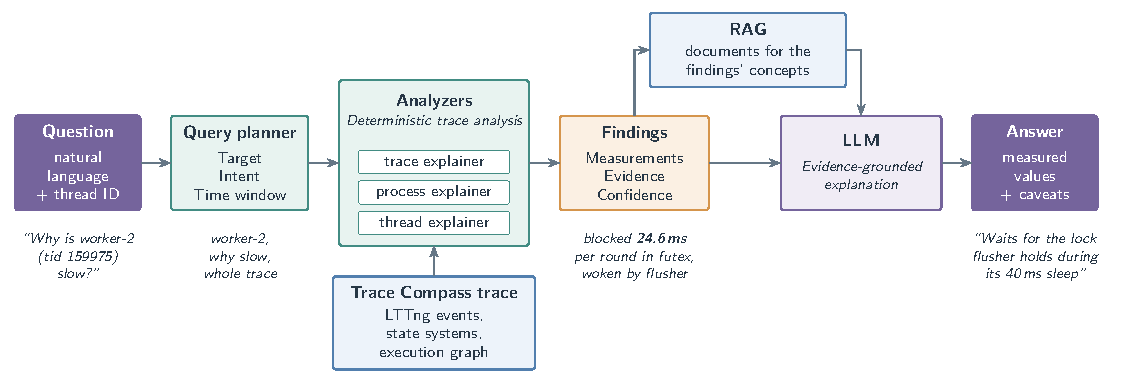
\includegraphics[width=\textwidth]{traceassist_pipeline}.
% Colours follow report/figures/unified_workflow.tex.
\documentclass[tikz,border=2mm]{standalone}
\usepackage[T1]{fontenc}
\usepackage{lmodern}
\usetikzlibrary{arrows.meta,positioning,calc}

\definecolor{ink}{HTML}{273746}
\definecolor{line}{HTML}{657786}
\definecolor{purple}{HTML}{75649C}
\definecolor{teal}{HTML}{428C83}
\definecolor{blue}{HTML}{527FAE}
\definecolor{orange}{HTML}{D5954C}
\definecolor{greenfill}{HTML}{E8F3F0}
\definecolor{bluefill}{HTML}{EDF3FA}
\definecolor{lavender}{HTML}{F0ECF5}
\definecolor{orangefill}{HTML}{FBF0E3}

% Box heading, and the role tag under it.
\newcommand{\hd}[1]{{\bfseries\fontsize{8.5}{10}\selectfont #1}}
\newcommand{\role}[1]{{\itshape\fontsize{7}{8.5}\selectfont #1}}

\begin{document}
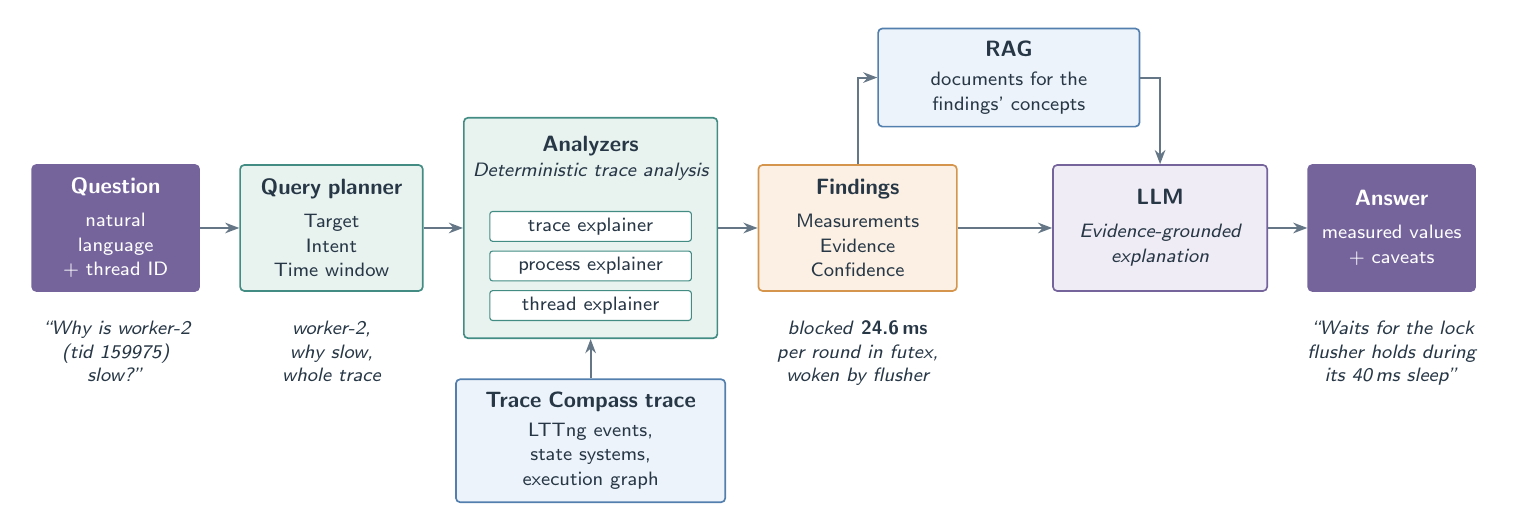
\begin{tikzpicture}[
  font=\sffamily\fontsize{7.5}{9}\selectfont, text=ink,
  box/.style={draw, rounded corners=1.5pt, align=center, inner sep=1.6mm,
              line width=.6pt, minimum height=16mm},
  flow/.style={draw=line, line width=.7pt, -{Stealth[length=1.8mm]}},
  example/.style={font=\sffamily\itshape\fontsize{7}{8.5}\selectfont, text=ink,
                  align=center, text width=#1, anchor=north},
  node distance=5mm and 5mm]

% ---- main flow -----------------------------------------------------------
\node[box, draw=purple, fill=purple, text=white, text width=18mm] (q)
  {\hd{Question}\\[1mm] natural language\\ + thread ID};

\node[box, draw=teal, fill=greenfill, text width=20mm, right=of q] (plan)
  {\hd{Query planner}\\[1mm] Target\\ Intent\\ Time window};

% Analyzers: one box holding the three explainers.
\node[box, draw=teal, fill=greenfill, text width=29mm, right=of plan,
      minimum height=28mm] (an) {};
\node[anchor=north, align=center] at ($(an.north)+(0,-1.2mm)$)
  {\hd{Analyzers}\\ \role{Deterministic trace analysis}};
\node[draw=teal, fill=white, rounded corners=1pt, text width=24mm, align=center,
      inner sep=.8mm] (te) at ($(an.center)+(0,0.2mm)$) {trace explainer};
\node[draw=teal, fill=white, rounded corners=1pt, text width=24mm, align=center,
      inner sep=.8mm, below=1.1mm of te] (pe) {process explainer};
\node[draw=teal, fill=white, rounded corners=1pt, text width=24mm, align=center,
      inner sep=.8mm, below=1.1mm of pe] (th) {thread explainer};

\node[box, draw=orange, fill=orangefill, text width=22mm, right=of an] (fd)
  {\hd{Findings}\\[1mm] Measurements\\ Evidence\\ Confidence};

\node[box, draw=purple, fill=lavender, text width=24mm, right=12mm of fd] (llm)
  {\hd{LLM}\\[1mm] \role{Evidence-grounded}\\ \role{explanation}};

\node[box, draw=purple, fill=purple, text=white, text width=18mm, right=of llm] (ans)
  {\hd{Answer}\\[1mm] measured values\\ + caveats};

% ---- inputs and retrieval ------------------------------------------------
\node[box, draw=blue, fill=bluefill, text width=31mm, minimum height=10mm,
      below=5mm of an] (tr)
  {\hd{Trace Compass trace}\\[.5mm] LTTng events, state systems,\\ execution graph};

\node[box, draw=blue, fill=bluefill, text width=30mm, minimum height=10mm]
  (rag) at ($(fd.north)!.5!(llm.north)+(0,11mm)$)
  {\hd{RAG}\\[.5mm] documents for the\\ findings' concepts};

% ---- arrows --------------------------------------------------------------
\draw[flow] (q) -- (plan);
\draw[flow] (plan) -- (an);
\draw[flow] (an) -- (fd);
\draw[flow] (fd) -- (llm);
\draw[flow] (llm) -- (ans);
\draw[flow] (tr) -- (an);
\draw[flow] (fd.north) |- (rag.west);
\draw[flow] (rag.east) -| (llm.north);

% ---- worked example (Q5, 2-minute trace), all on one row -----------------
\coordinate (ex) at ($(plan.south)+(0,-2.5mm)$);
\node[example=20mm] at (q |- ex)
  {``Why is worker-2\\ (tid 159975) slow?''};
\node[example=22mm] at (plan |- ex)
  {worker-2,\\ why slow,\\ whole trace};
\node[example=24mm] at (fd |- ex)
  {blocked \textbf{24.6\,ms}\\ per round in futex,\\ woken by flusher};
\node[example=26mm] at (ans |- ex)
  {``Waits for the lock\\ flusher holds during\\ its 40\,ms sleep''};

\end{tikzpicture}
\end{document}
